\section{Введение}

Смартфоны -- неотъемлемая часть жизни любого современного человека. С их помощью люди общаются, делают снимки, организуют поездки, делают покупки, следят за новостями. За развитием смартфонов следит буквально весь мир -- из года в год добавляются всё новые функции и возможности. \\

Одной из таких показательных функций является способность смартофона с большой точностью определять угол поворота телефона и вычислять ускорение с помощью встроенных акселерометра и гироскопа. Однако эти приборы не так часто используются -- разве что для ориентации изображения на экране, подсчете шагов в приложениях для спорта и управления в некоторых играх. \\

В рамках данной работы перед командой была поставлена цель -- разработать технологию, позволяющую распознавать различные движения и жесты, совершаемые с помощью мобильного телефона. Для достижения это цели были поставлены глобальные задачи:

\begin{itemize}
    \item Разработать мобильное приложения для сбора данных и тестирования, распознавания и восстановления движений.
    \item Разработать механизм классификации записей отдельного такта движения с акселерометра.
    \item Разработать библиотеку для мобильных устройств, позволяющую в любое приложение интегрировать управление с помощью жестов.
    \item Создать механизм выделения отдельных тактов движения в timeseries акселерометра.
    \item Создать восстановления движения по акселерометру и гироскопу.
    \item Создать механизм сглаживания и фильтрации данных акселерометра и гироскопа
\end{itemize}

\section{Обзор и сравнительный анализ источников по теме проекта \\ (Гусев Владислав)}

Одной из задач являлось исследование уже существующих решений по классификации движений или жестов. Поиск осуществлялся во всех открытых источниках. В свободном доступе готовых решений почти что нет. Поэтому данная задача заняла достаточно большое количество времени.

Считаю нужным отметить, что нас устраивают алгоритмы, которые работают только с аппаратными составляющими – акселерометром и гироскопом.

Сразу можно разделить алгоритмы по распознаванию жестов на 2 категории:

\begin{itemize}
    \item классификация по 3D графику или 3D фигуре.
    \item классификация по некому внешнему подобию 3D фигуры (в нашем случае 2D проекции 3D фигуры)
\end{itemize}

Но методы, использующие 3D модель для идентификации жестов, обрабатывают сложные трехмерные поверхности и классифицируют жесты с помощью нейронных сетей. Следовательно, недостатком такого метода является большая ресурсоемкость, так как построение самой модели, обучение нейронной сети и ее использование могут потребовать значительных ресурсов, что недопустимо при разработке технологии для мобильных устройств. Поэтому было принято решение оставить классификацию движений по 2D проекции.

Далее были выявлены классы, на которые деляется алгоритмы по распознаванию 2D жестов или движений:

\begin{itemize}
    \item основывающиеся на шаблонах – их суть в том, что они хранят эталонные движения или жесты, а далее производится их сравнение с произведенным движением при помощи различных метрик.
    \item основывающиеся на моделях -- содержат в себе нахождение и выделение основных характеристик в поступающих данных и классификация этих характеристик.
\end{itemize}

К первому классу относится алгоритм uWave. Данный алгоритм использует только показания акселерометра, но  заявлена точность в $95 \%$, что жест будет распознан правильно.
Данный алгоритм соответствует своей точности только при исследовании 8 различных жестов:

\begin{figure}[H]
    \begin{center}
        \begin{tabular}{ccc}
            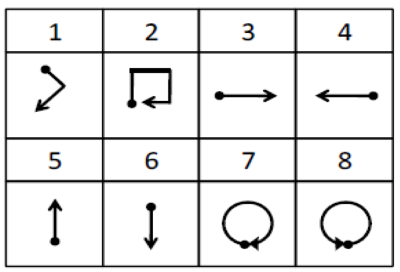
\includegraphics[scale = 0.9]{images/uWave_1.png} & 
            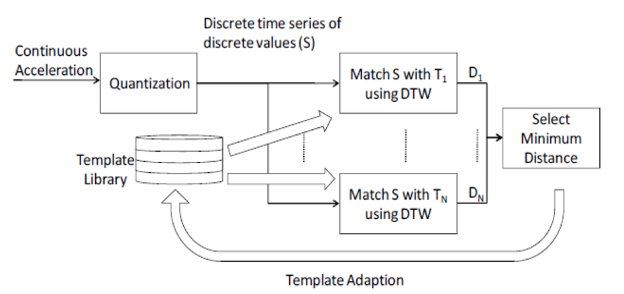
\includegraphics[scale = 0.9]{images/uWave_2.png} \\
        \end{tabular}
    \end{center}
\end{figure}

Теперь рассмотрим более детально данный алгоритм: \\
Его можно разбить на 3 части:
\begin{itemize}
    \item квантования данных, полученных с акселерометра.
    \item подбор соответствующего шаблона движения.
    \item адаптация шаблона (на рисунке ниже представлена более детальная схема работы).
\end{itemize}

Основной частью в алгоритме является другой алгоритм, называющийся «Динамической Трансформацией шкалы времени» («Dynamic Time Warping») -- он позволяет сравнить две последовательности (причем он может учитывать скорость изменения данных), например, данных алгоритм часто используют для распознавания речи. Если же более детально посмотреть на алгоритм «DTW», то он находит расстояние Левенштейна между последовательностью, записанной текущим жестом, и последовательностью эталонного жеста.

Последним шагом алгоритма является адаптация шаблона. Так как способ реализации жеста меняется от времени к времени, даже если этот жест будет исполнять один и тот же человек, следовательно нам нужно постоянно корректировать эталонный жест. Поэтому применяется незамысловатый алгоритм для поддержания актуальности жестов: для каждого эталона мы храним по две вариации его исполнения, и каждый новый способ, удачно распознанный, заменяет более старый из уже существующих двух.

Также стоит рассмотреть статические методы распознавнаия движений:
\begin{itemize}
    \item Например, Скрытие Марковские Цепи, который базируется на вероятностной интерпретации эталонов жестов для моделирования траектории жеста. При этом перед тем, как запустить алгоритм, следует провести предобработку входящих данных двумя фильтрами: первый -- отбрасывает вектора данных, которые не вносят значимый вклад в характеристику движения или жеста, второй – устраняет векторы данных, которые примерно похожи на предыдущий. Данный алгоритм неправильно классифицирует около $4-5 \%$ моделей, то есть в $95-96 \%$  случаев мы получим правильный результат, что весьма неплохо.
    \item Также имеем достаточно популярный метод: метод опорных векторов. Его основная идея перевод исходных векторов в пространство большей размерности и нахождение разделяющей гиперплоскости с максимальным зазором в этом пространстве. Соответственно две параллельные гиперплоскости будут находиться по обе стороны от разделяющей гиперплоскости. (Но суть работы с жестами заключается в том, чтобы строить множество разделяющих гиперплоскостей, чтобы была возможность поступающий жест определить к своему классу). При этом точность данного метода может достигать $98 \%$.
\end{itemize}

Подводя итог данному анализу, можно скзаать, что знание внутреннего устройства схожих алгоритмов, уже дало нам информацию о надобности фильтрации входных данных, а также помогло ускорить реализацию различных частей, так как мы могли ориентироваться на готовые решения.